\documentclass[aspectratio=169,xcolor=dvipsnames]{beamer}
\usetheme[progressbar=frametitle,block=fill]{metropolis}
\title{Formal Software Verification Project Presentation}
\subtitle{SAT Solver}
\date{January 7, 2025}
\author{Nathan Schmidt}
\institute{Aarhus University}
\titlegraphic{
\includegraphics[scale=0.8]{aulogo.pdf}}

\usepackage{centernot}

\begin{document}
    \maketitle

    \begin{frame}{Syntax and Semantics}
        \begin{block}{Syntax}
            $$p, q ::= x\;|\;\texttt{true}\;|\;\texttt{false}\;|\;p \land q\;|\;p \lor q\;|\;p \rightarrow q\;|\;\neg p$$
            \vspace*{-20pt}
            \begin{itemize}
                \item Abstract: inductive type \texttt{form}
                \item Concrete: \texttt{Notation}
            \end{itemize}
        \end{block}

        \pause
        
        \begin{block}{Semantics}
            \begin{itemize}
                \item Valuation $v : \alert{\texttt{id}} \rightarrow \texttt{bool}$
                \item Interpreter $\texttt{interp} : \texttt{valuation} \times \texttt{form} \rightarrow \texttt{bool}$
            \end{itemize}
        \end{block}
    \end{frame}

    \begin{frame}{Simplifications}
        \small\begin{alignat*}{4}
            \texttt{true} \land p &\equiv p &p \land \texttt{true} &\equiv p &\texttt{false} \land p &\equiv \texttt{false}\hspace*{20pt}&p \land \texttt{false} &\equiv \texttt{false} \\
            \texttt{true} \lor p &\equiv \texttt{true}\hspace*{20pt}&p \lor \texttt{true} &\equiv \texttt{true}\hspace*{20pt}&\texttt{false} \lor p &\equiv p &p \lor \texttt{false} &\equiv p \\
            \texttt{true} \rightarrow p &\equiv p &p \rightarrow \texttt{true} &\equiv \texttt{true} &\texttt{false} \rightarrow p &\equiv \texttt{true} &p \rightarrow \texttt{false} &\equiv \neg p \\
            &&\neg \texttt{true} &\equiv \texttt{false} &\neg \texttt{false} &\equiv \texttt{true}
        \end{alignat*}
    \end{frame}

    \begin{frame}{Optimizer}
        \begin{columns}
            \column{0.45\textwidth} \begin{itemize}
                \item Syntax-driven
                \item Depth-First-Search (DFS):
                \begin{itemize}
                    \item[\textbf{X}] Pre-order: no obviously decreasing arguments
                    \item[$\checkmark$] \alert{Post-order}
                \end{itemize}
            \end{itemize}
            \column{0.55\textwidth}
            \begin{minipage}[t][\textheight][t]{\textwidth}
                \only<2>{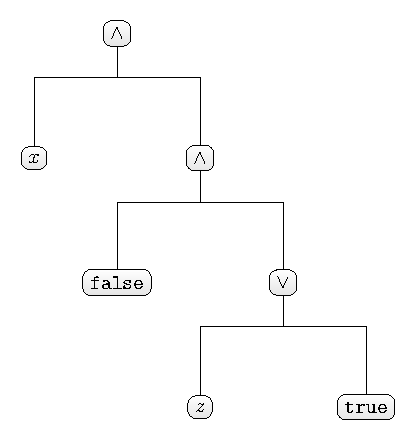
\includegraphics{figures/optimizer1.pdf}}
                \only<3>{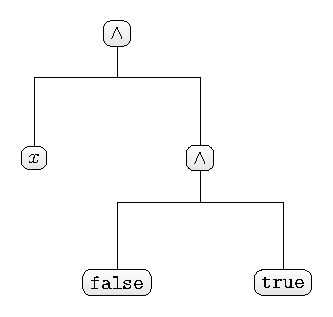
\includegraphics{figures/optimizer2.pdf}}
                \only<4>{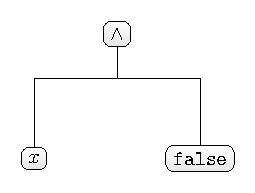
\includegraphics{figures/optimizer3.pdf}}
                \only<5>{\hspace*{32pt}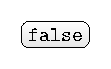
\includegraphics{figures/optimizer4.pdf}}   
            \end{minipage}
        \end{columns}
    \end{frame}

    \begin{frame}{Optimizer Correctness and Minimality}
        \begin{block}{Correctness}
            \textbf{Theorem.}\hspace*{8pt}\emph{$\forall\,v, p : \texttt{interp}\;v\;p = \texttt{interp}\;v\;(\texttt{optim}\;p)$}
        \end{block}

        \pause

        \begin{block}{Minimality}
            \begin{itemize}
                \item $p$ in \alert{minimal form}:
                    \begin{itemize}
                        \item if $p = \texttt{true}$/\texttt{false}, or
                        \item \texttt{true}/\texttt{false} $\notin p \pause \leadsto$ inductive predicate
                    \end{itemize}
                \pause
                \item \textbf{Theorem.}\hspace*{8pt}\emph{\texttt{optim $p$} always in minimal form}
            \end{itemize}
        \end{block}
    \end{frame}

    \begin{frame}{Solver}
        \begin{center}
            \scalebox{0.8}{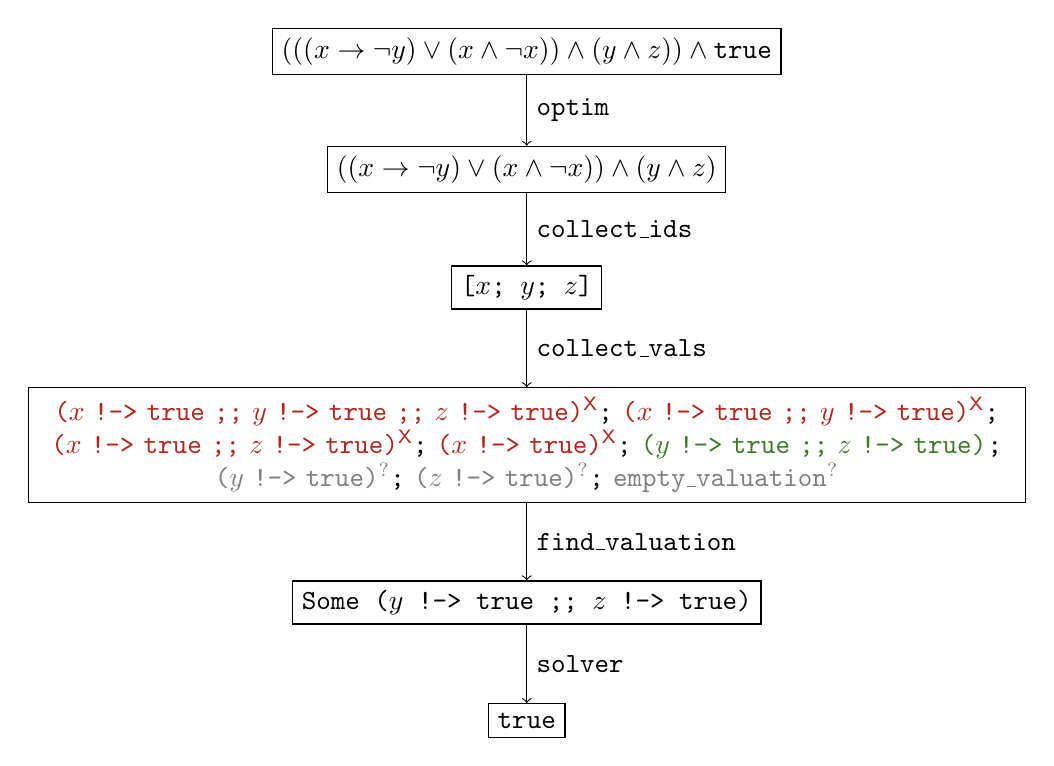
\begin{tikzpicture}
                \node[draw] (step1) at (0,0) {$(((x \rightarrow \neg y) \lor (x \land \neg x)) \land (y \land z)) \land \texttt{true}$};
                \onslide<2->{\node[draw] (step2) at (0,-1.5) {$((x \rightarrow \neg y) \lor (x \land \neg x)) \land (y \land z)$};}
                \onslide<3->{\node[draw] (step3) at (0,-3) {\texttt{[$x$; $y$; $z$]}};}
                \onslide<4->{\node[draw] (step4) at (0,-5) [text width=1.025\textwidth,align=center]{\texttt{\textcolor{BrickRed}{($x$ !-> true ;; $y$ !-> true ;; $z$ !-> true)$^\mathsf{X}$}; \textcolor{BrickRed}{($x$ !-> true ;; $y$ !-> true)$^\mathsf{X}$}; \textcolor{BrickRed}{($x$ !-> true ;; $z$ !-> true)$^\mathsf{X}$}; \textcolor{BrickRed}{($x$ !-> true)$^\mathsf{X}$}; \textcolor{OliveGreen}{($y$ !-> true ;; $z$ !-> true)$^{\checkmark}$};\\ \textcolor{gray}{($y$ !-> true)$^\mathsf{?}$}; \textcolor{gray}{($z$ !-> true)$^\mathsf{?}$}; \textcolor{gray}{empty\_valuation$^\mathsf{?}$}}};}
                \onslide<5->{\node[draw] (step5) at (0,-7) {\texttt{Some ($y$ !-> true ;; $z$ !-> true)}};}
                \onslide<6>{\node[draw] (step6) at (0,-8.5) {\texttt{true}};}

                \onslide<2->{\path[->] (step1) edge node[midway, right]{\texttt{optim}} (step2);}
                \onslide<3->{\path[->] (step2) edge node[midway, right]{\texttt{collect\_ids}} (step3);}
                \onslide<4->{\path[->] (step3) edge node[midway, right]{\texttt{collect\_vals}} (step4);}
                \onslide<5->{\path[->] (step4) edge node[midway, right]{\texttt{find\_valuation}} (step5);}
                \onslide<6->{\path[->] (step5) edge node[midway, right]{\texttt{solver}} (step6);}
            \end{tikzpicture}}
        \end{center}
    \end{frame}

    \begin{frame}{Solver Soundness and Completeness}
        \begin{block}{Soundness}
            \begin{itemize}
                \item \textbf{Lemma.}\hspace*{8pt}\emph{$\forall\,p :$ \texttt{solver $p =$\,true} $\Longrightarrow$ \texttt{satisfiable $p$}}
                \item Proof by induction
                \item Do \alert{not} care about \alert{exact} returned valuation
            \end{itemize}
        \end{block}

        \pause

        \begin{block}{Completeness}
            \begin{itemize}
                \item \textbf{Lemma.}\hspace*{8pt}\emph{$\forall\,p :$ \texttt{satisfiable $p$} $\Longrightarrow$ \texttt{solver $p =$\,true}}
                \item \texttt{interp $v$ $p =$\,true $\alert{\centernot\Longrightarrow} v \in$ collect\_vals\,(collect\_ids $p$))}
                \pause
                \item Proof attempt:
                \begin{itemize}
                    \item $\forall\,v, v' : \forall\,x \in p, v\,x = v'\,x \Longrightarrow$ \texttt{interp} $v$ $p =$ \texttt{interp} $v'$ $p$
                    \item $\forall v : \exists v' : \forall\,x \in p, v\,x = v'\,x$ and $v' \in$ \texttt{collect\_vals\,(collect\_ids $p$))} 
                \end{itemize}
            \end{itemize}
        \end{block}
    \end{frame}

    \begin{frame}{Solver Decision Procedure}
        \begin{theorem}
            $\forall\,p :$ \texttt{solver $p =$true} $\Longleftrightarrow$ \texttt{satisfiable $p$}
        \end{theorem}

        \pause
        
        \begin{center}
            \Large i.e., \texttt{solver} decision procedure for SAT
        \end{center}
    \end{frame}
\end{document}